\documentclass[conference]{IEEEtran}
\IEEEoverridecommandlockouts
% The preceding line is only needed to identify funding in the first footnote. If that is unneeded, please comment it out.
\usepackage{cite}
\usepackage{amsmath,amssymb,amsfonts}
\usepackage{algorithmic}
\usepackage{graphicx}
\usepackage{textcomp}
\usepackage{xcolor}
\def\BibTeX{{\rm B\kern-.05em{\sc i\kern-.025em b}\kern-.08em
    T\kern-.1667em\lower.7ex\hbox{E}\kern-.125emX}}
\begin{document}


\title{Arduino based Smart Cricket Stadiun}

\author{\IEEEauthorblockN{Md Shafayet Hossain Ovi\IEEEauthorrefmark{1}, Md Tashin Parvez
\IEEEauthorrefmark{2}, Md Azizul Hoque Noman\IEEEauthorrefmark{3}, Sharmin Sultana
\IEEEauthorrefmark{4},Md Musfiqur Rahman\IEEEauthorrefmark{5}}
\IEEEauthorblockA{\textit{Dept. of Computer Science and Engineering} \\
\textit{United International University, Dhaka, Bangladesh}\\
011221385\IEEEauthorrefmark{1}, 011221437\IEEEauthorrefmark{2},
011221338\IEEEauthorrefmark{3}, 011221331\IEEEauthorrefmark{4} and 011221334\IEEEauthorrefmark{5}
}}

\maketitle


\begin{abstract}
This report is about to an electronic hardware based project where we have implemented an Arduino based Smart Cricket Stadium. 
Our aim is to make cricket games more efficient during unstable weather by implementing an automated pitch covering system. To make this report understandable,
We added a flowchart, photographs, and descriptions. Our features can also be applicable in other places.
\end{abstract}

\begin{IEEEkeywords}
 Arduino,HDS,Stepper Motor, LDR, Servo, IR
\end{IEEEkeywords}


\section{Project Overview }
Our project is about an Arduino-based smart cricket stadium. The reason we implemented this project was to make cricket more automated and accurate. We also ensure that our automated feature is suitable during playtime. We secure the pitch to be dry during rain time so that the play may start after the rain using HDS and Stepper Motor. Also, we placed the boundary line after displacement by fielders or others. To  detect that the line is displace we use weight sensor and fixed the line using DC Motor Mechanism. And to ensure the power play rules, we get count from IR sensor that how many players are inside 30 yards and outside 30 yards . This will help the umpire make the correct decision. Another feature is control stadium light brightness according sunlight based on LDR sensor read. Apart from this we implement move able solar system according sun position to absorb maximum power using servo motor and LDR sensor.

\begin{figure}
    \centering
    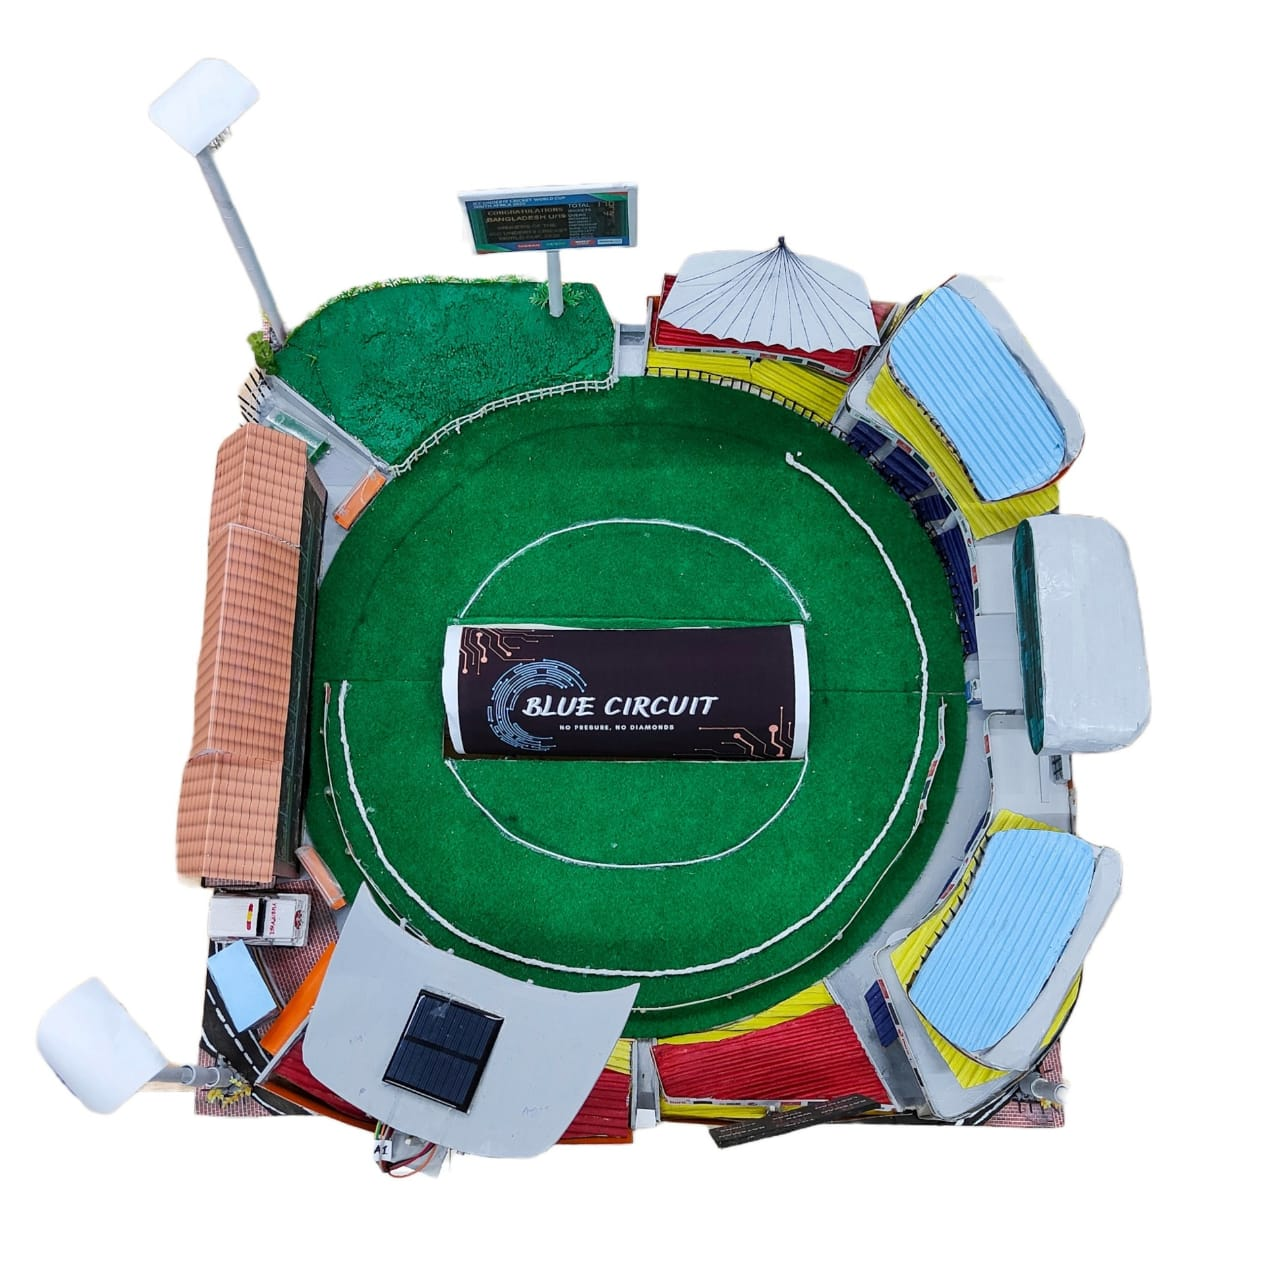
\includegraphics[width=3in]{BlueCircuit.jpg}
    \caption{Project picture}
    \label{fig:ultrasonicl}
\end{figure}

\section{Component List}


\begin{enumerate}
    \item Arduino Uno
    \item Humidity Detection Sensor
    \item  Stepper Motor
    \item LDR Sensor
    \item Servo Motor
    \item IR Sensor
    \item DC Motor
    \item Resistor
    \item Jumper Wire
    \item Solar Panel
    \item Li-ion Battery
    \item Rain sensor
\end{enumerate}

\subsection{Arduino UNO}

 Adiouno is an open-source electronics microcontroller board based on the ATmega328P. This board is able to read input (from many sensors) and turn it into an output. It has three ports: B (digital pins 8 to 13), C (analog input pins), and D (digital pins 0 to 7). And it contains six analog inputs, a 16 MHz ceramic resonator, 14 digital input/output pins (six of which can be used as PWM outputs), a USB port, a power jack, an ICSP header, and a reset button. It comes with everything needed to support the microcontroller; to get started, just plug in a USB cable, an AC-to-DC adapter, or a battery. The open-source, programmable Arduino UNO microcontroller board is inexpensive, adaptable, and simple to use, and it may be used in a number of electronic projects.
 
\begin{figure}
    \centering
    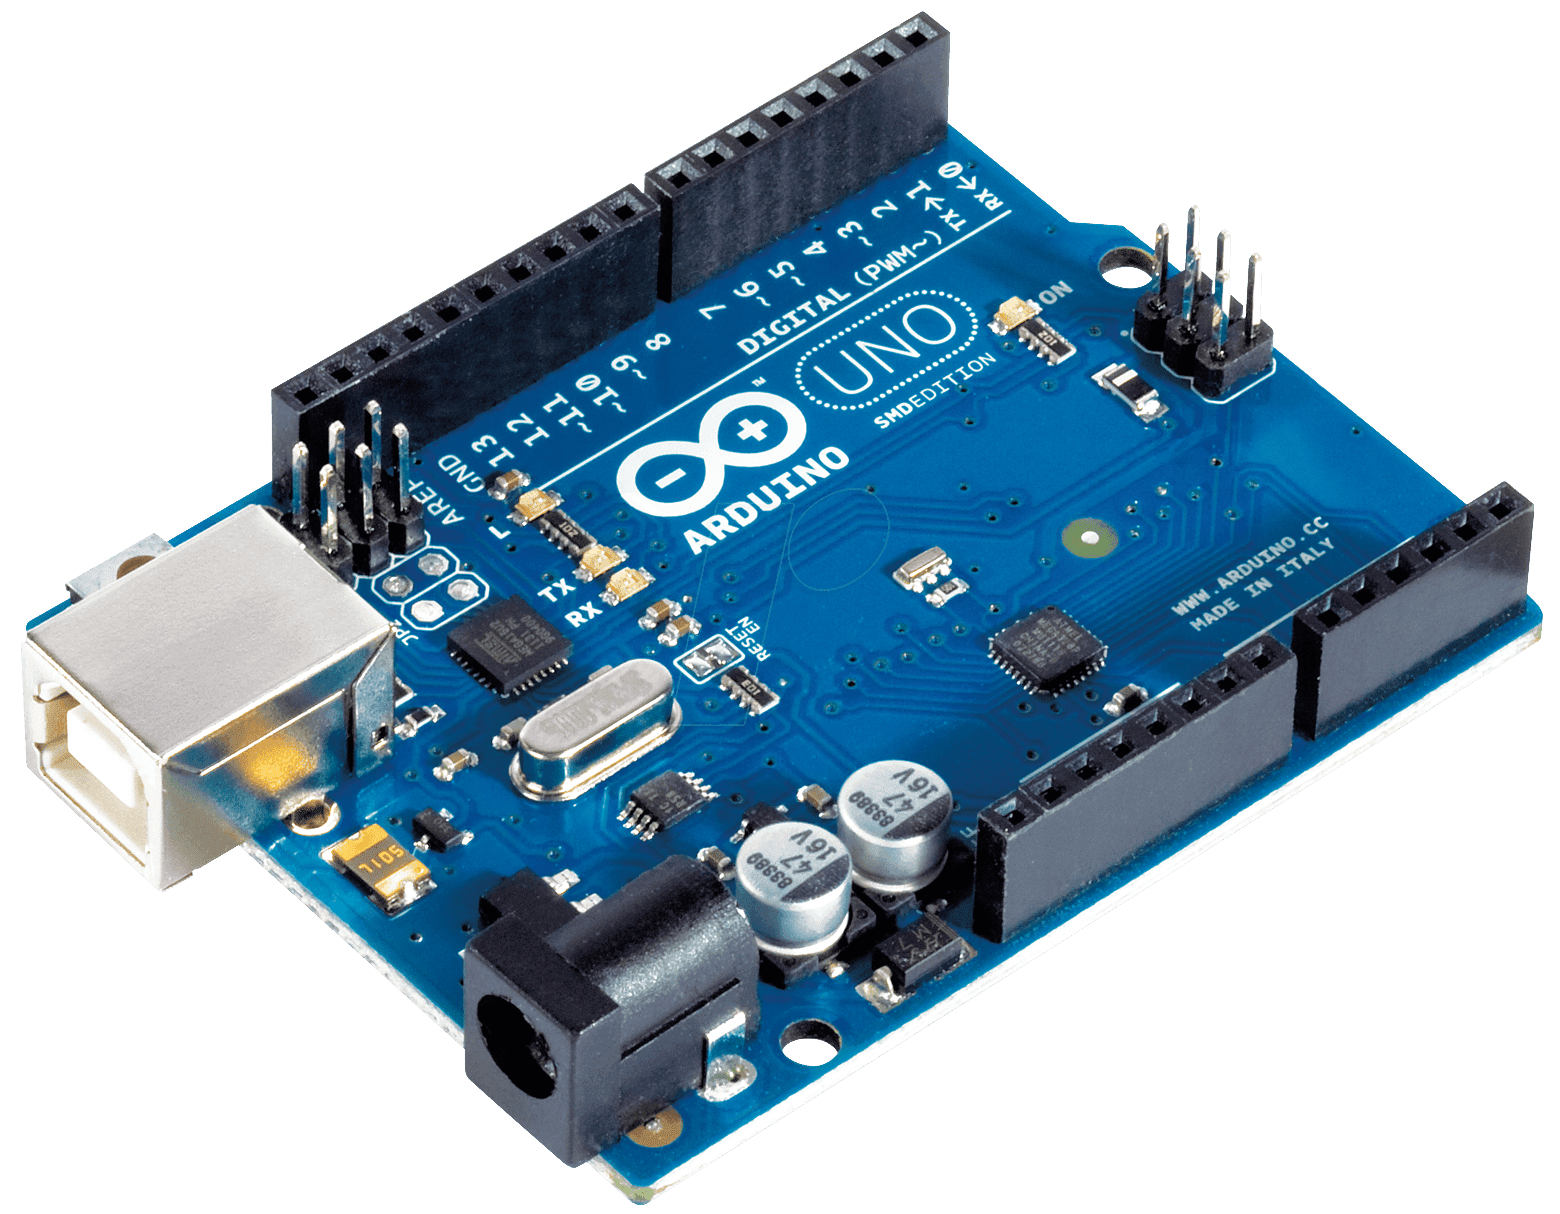
\includegraphics[width=0.5\linewidth]{Arduino Image.png}
    \caption{Arduino Image}
    \label{fig:enter-label}
\end{figure}
\subsection{Servo Motor}
\begin{figure}
    \centering
    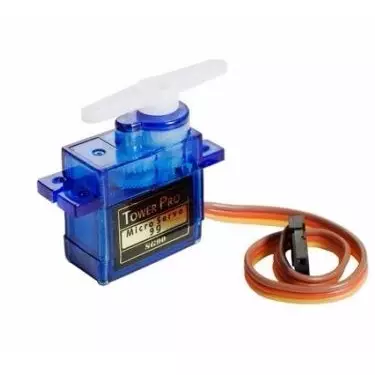
\includegraphics[width=0.5\linewidth]{Servo.png}
    \caption{Servo Motor}
    \label{fig:enter-label}
\end{figure}


A type of motor that helps things move with precision is called a servo motor. It is used where things need to move or rotate at a certain angle or distance. It runs through a servo mechanism with a simple motor. It is called an AC servo motor when it gets AC power; it is also called DC power when it gets DC power.
 It was used to create simple robots, remote-controlled cars, etc. because in this kind of system we need to rotate an arm or wheel at a certain angle and take it back to its previous position. 
 


\subsection{Humidity Detection Sensor}
\begin{figure}
    \centering
    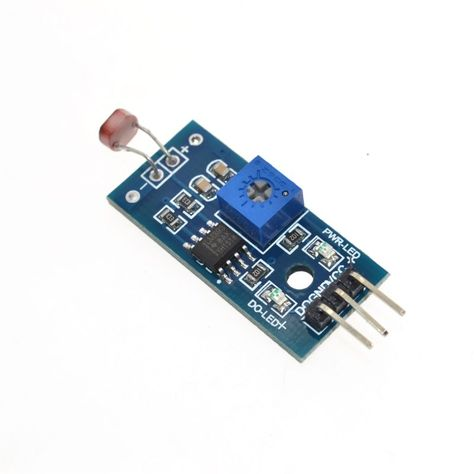
\includegraphics[width=0.5\linewidth]{Humidity Detection Sensor.png}
    \caption{Humidity Detection Sensor}
    \label{fig:enter-label}
\end{figure}
HDS is a small device that can detect a certain amount of water vapour or moisture in the air. It has a special material that changes its properties when it gets humid and reacts in a way that the sensor can detect. This sensor is capable of measuring if the air is dry (low humidity) or damp (high humidity). It can show us the level of humidity, so you can know if it's a humid day or a dry one.

\subsection{DC Motor}
\begin{figure}
     \centering
     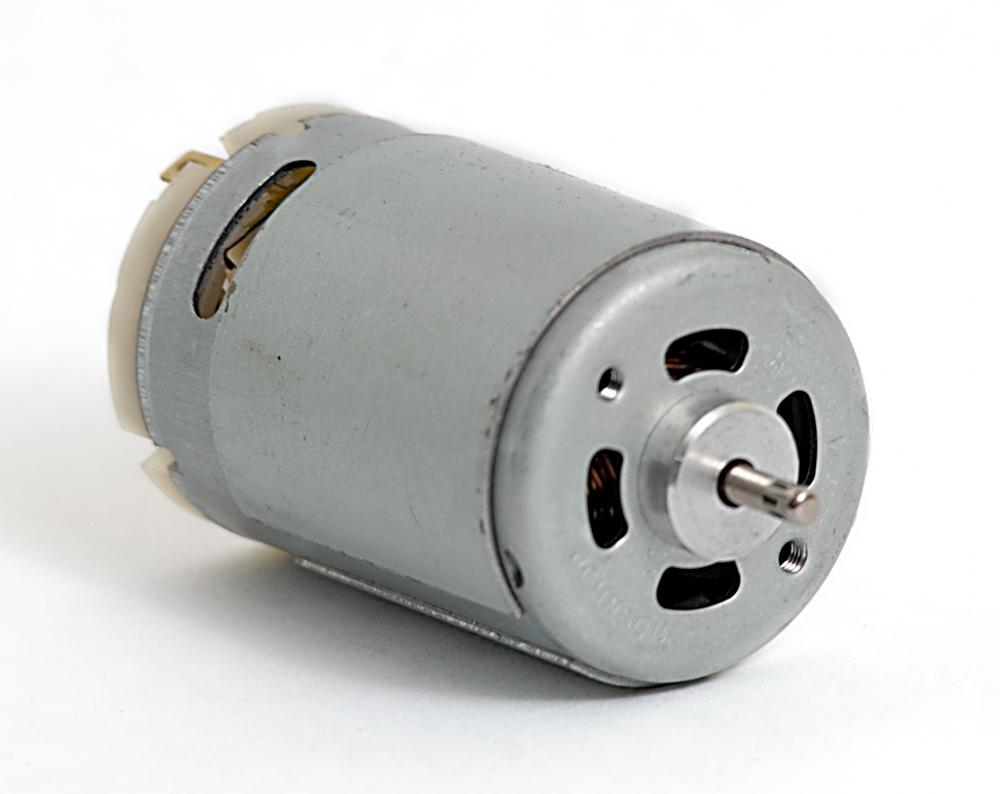
\includegraphics[width=0.5\linewidth]{DC Motor.png}
     \caption{DC Motor}
     \label{fig:enter-label}
 \end{figure} 
A DC motor is an electrical device that generates force through the use of direct current (DC). The most popular kinds depend on magnetic forces generated by currents in the coils. For a portion of the motor's current to occasionally shift direction, almost all types of DC motors contain an internal mechanism that is either electromechanical or electronic.

                 
\subsection{Li Battery}
\begin{figure}
    \centering
    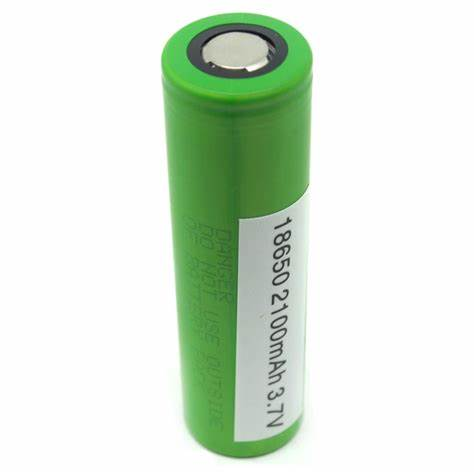
\includegraphics[width=0.5\linewidth]{Li Battery.png}
    \caption{Li Battery}
    \label{fig:enter-label}
\end{figure}
A lithium-ion battery is a rechargeable battery. It uses the reversible reduction of lithium ions, which store energy. The negative electrode of a lithium-ion cell is simply graphite, which is a form of carbon. The positive electrode is a metal oxide. Positive and negative celectrodes continue to exist in normal use. This electrolyte carries positively charged lithium ions from the anode to the cathode and from the cathode to the anode through the separator. The movement of the lithium ions creates free electrons in the anode and creates a charge at the positive current collector. 

\subsection{LDR Sensor}
\begin{figure}
    \centering
    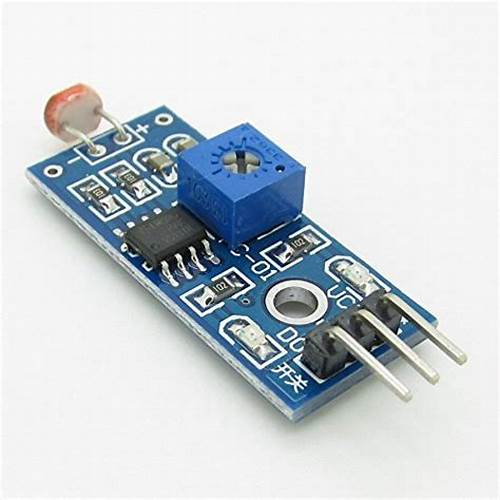
\includegraphics[width=0.5\linewidth]{image.png}
    \caption{LDR Sensor}
    \label{fig:enter-label}
\end{figure}

LDR (Light Dependent Resistor) is a special type of resistor. It helps us to direct the sunlight power and we identify is it dark or bright. We can use LDR sensors in many things, for example streetlights that turn on when it gets dark and off when it's bright, also in camera so that camera can get better light to produce better photo.
 

\subsection{Stepper Motor}
\begin{figure}
    \centering
    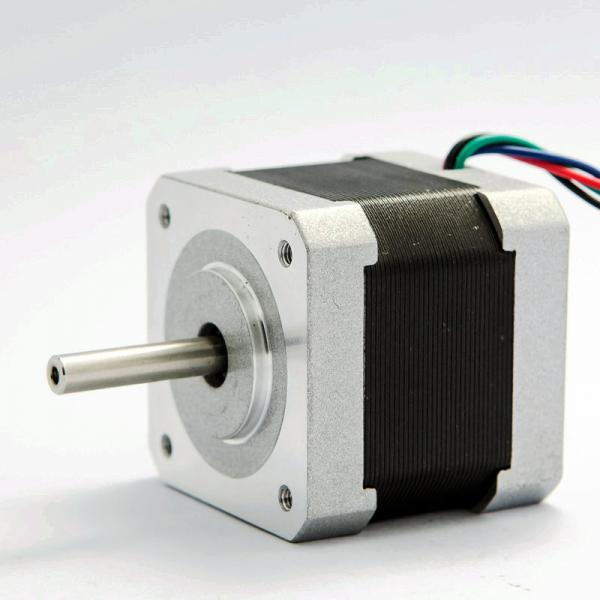
\includegraphics[width=0.5\linewidth]{Stepper Motor.png}
    \caption{Stepper Motor}
    \label{fig:enter-label}
\end{figure}

A brushless DC electric motor that divides a full rotation into a number of equal steps is referred to as a stepper motor, also known as a step motor or stepping motor. This electric motor that progresses by a predetermined number of degrees or turns its shaft in steps.
This trait, which results from the internal design of the motor, makes it possible to determine the precise angular position of the shaft by simply counting the number of steps made without the need of a sensor. Usually , its used in roted a component in left or right.


\subsection{Solar Panel}
\begin{figure}
    \centering
    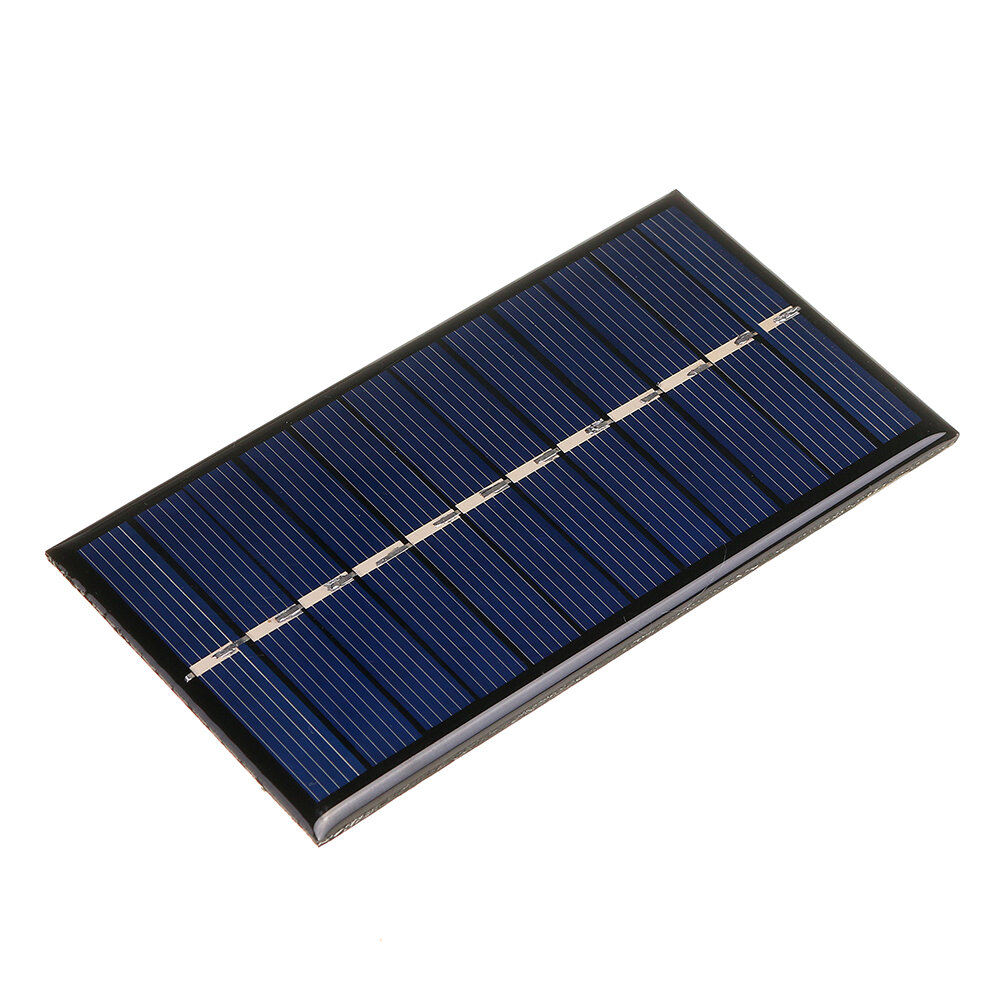
\includegraphics[width=0.5\linewidth]{Solar Panel.png}
    \caption{Solar Panel}
    \label{fig:enter-label}
\end{figure}
Solar Panel is a device that can generate electricity from sunlight. It is made by photovoltaic cells that can  produce electrones, when exposed to light. It's ideal for powering small devices, charging batteries, or demonstrating solar energy.

\subsection{Jumper Wire}
\begin{figure}
    \centering
    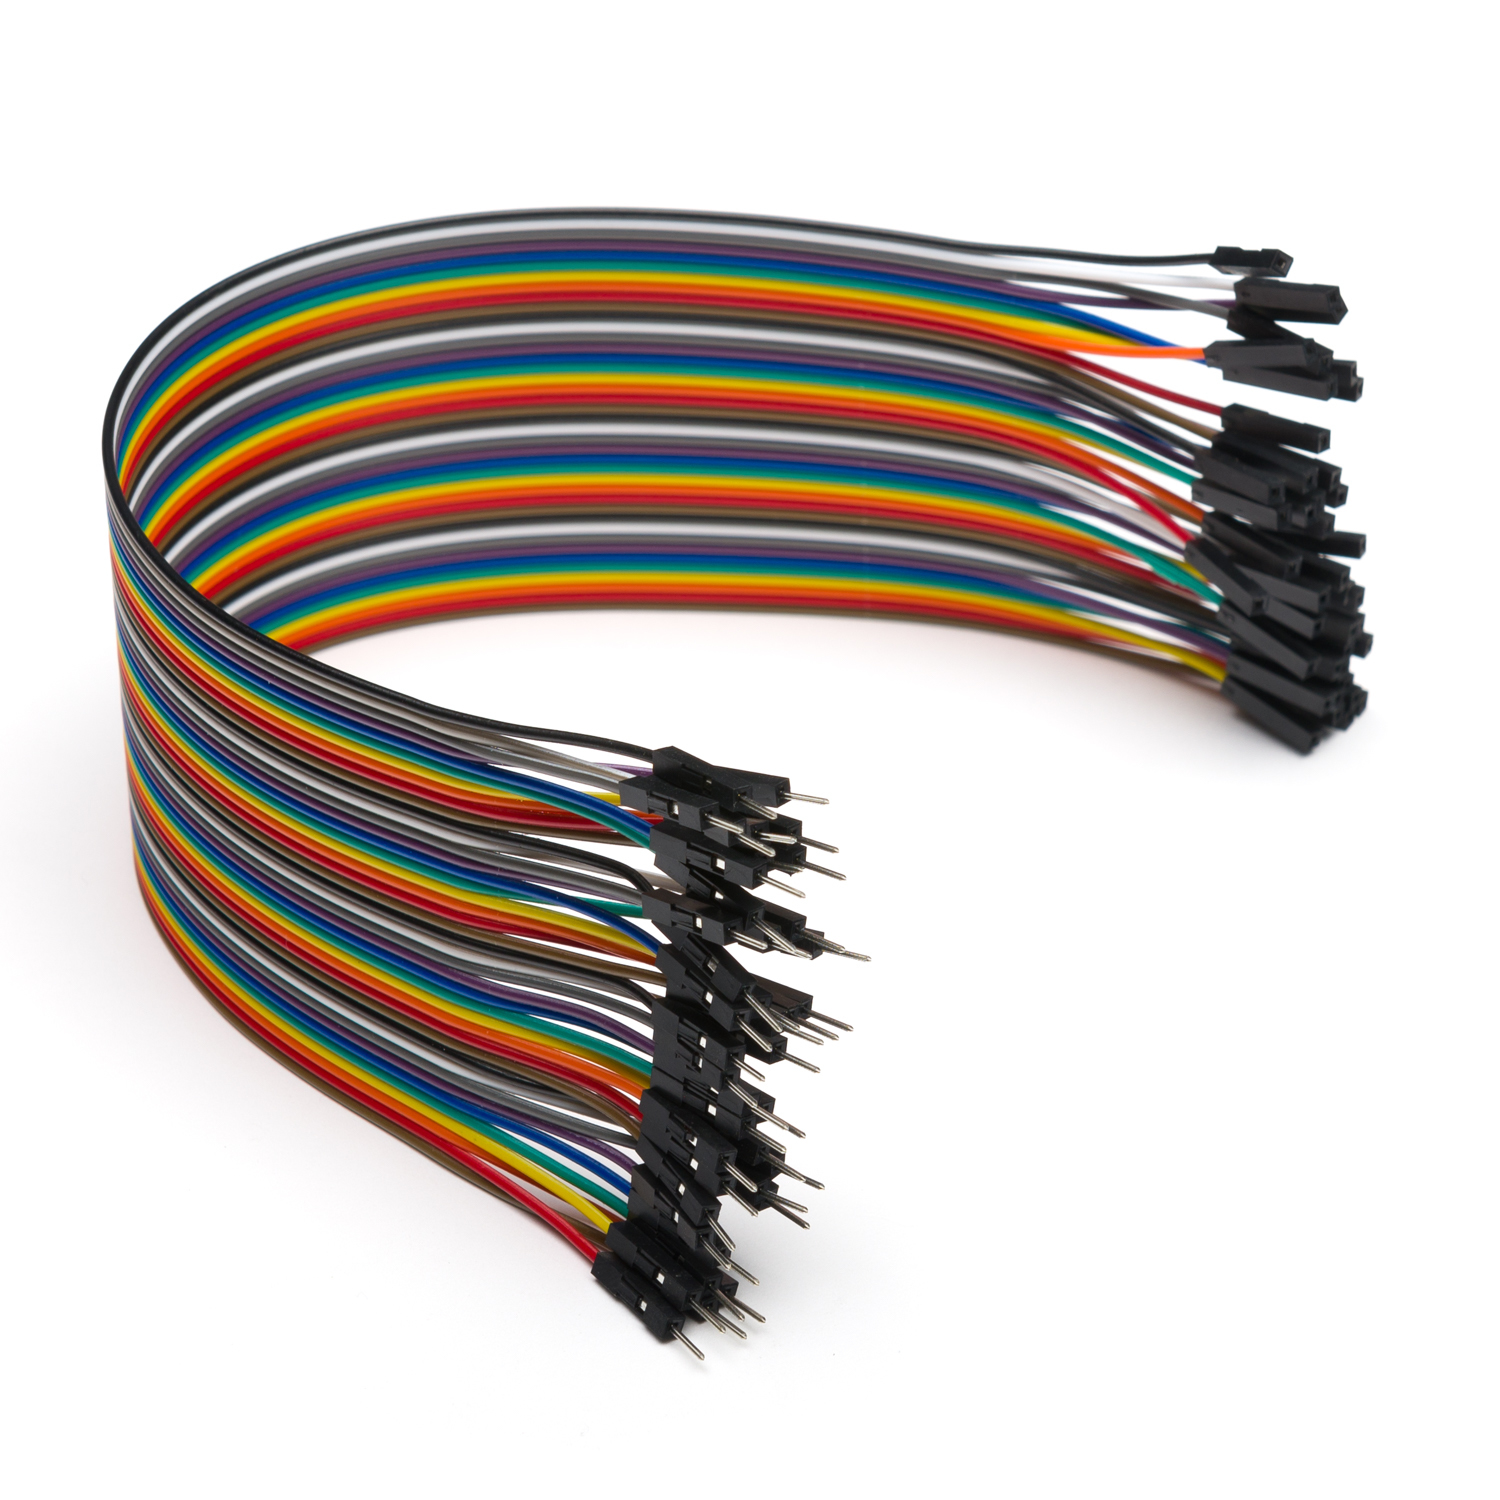
\includegraphics[width=0.5\linewidth]{Wire.png}
    \caption{Jumper Wire}
    \label{fig:enter-label}
\end{figure}
Jumper wire works as a road in any electronics project. It’s thin and flexible, too. This wire comes in two types: male and female. It was used to connect multiple electrical components like sensors, LEDs, Arduinos, batteries, etc. It is found in different colours so that we can easily identify which wire is used in which part of that component. It's a very common and essential tool because it connects multiple systems.



\subsection{Resistor}
\begin{figure}
    \centering
    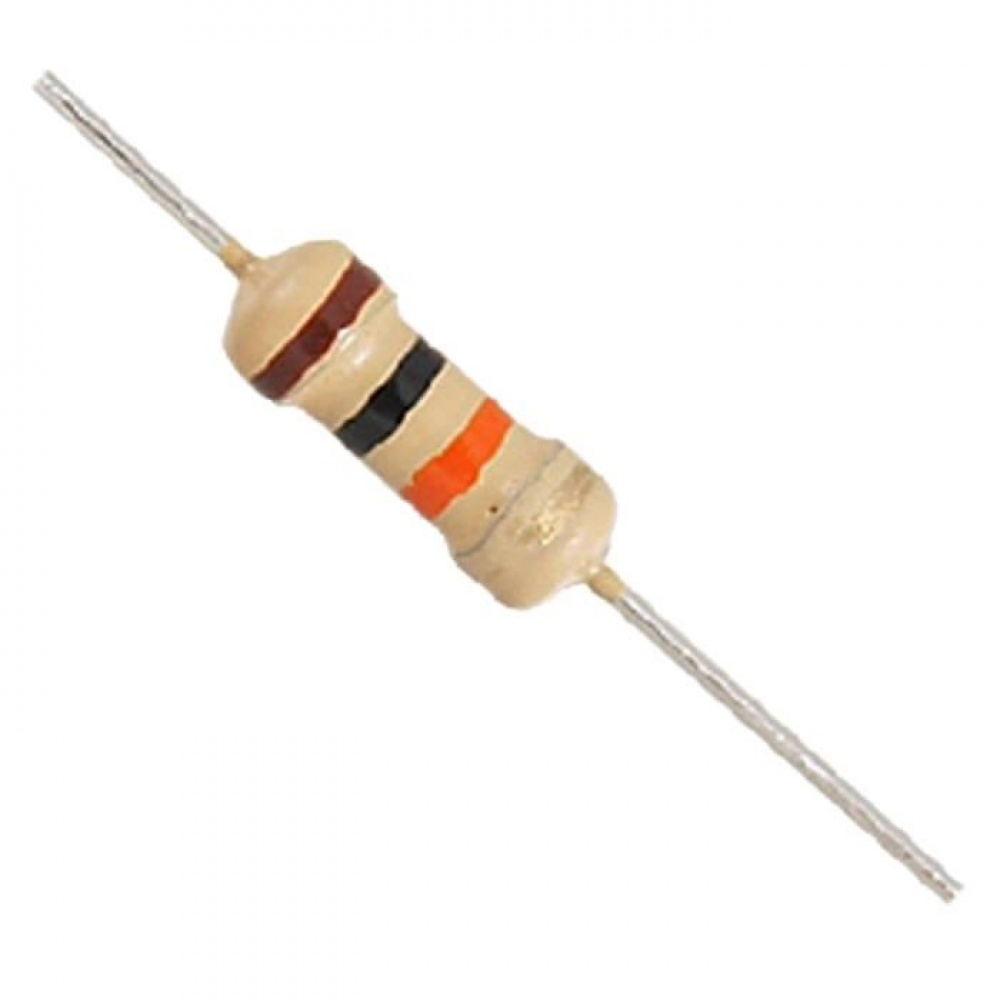
\includegraphics[width=0.5\linewidth]{Resistor.png}
    \caption{Resistor}
    \label{fig:enter-label}
\end{figure}
A resistor is a two-terminal component. It impalements electrical resistance as a circuit element. Resistors are used to minimize the adjust signal levels, current flow to divide voltages, terminate transference lines and many other uses. The resistor absorbs the electrical energy in the process where it acts as a hindrance to the flow of electricity by reducing the voltage, and it is dissipated as heat. A resistor limits current and dorps the voltage.

\subsection{IR Sensor}

\begin{figure}
    \centering
    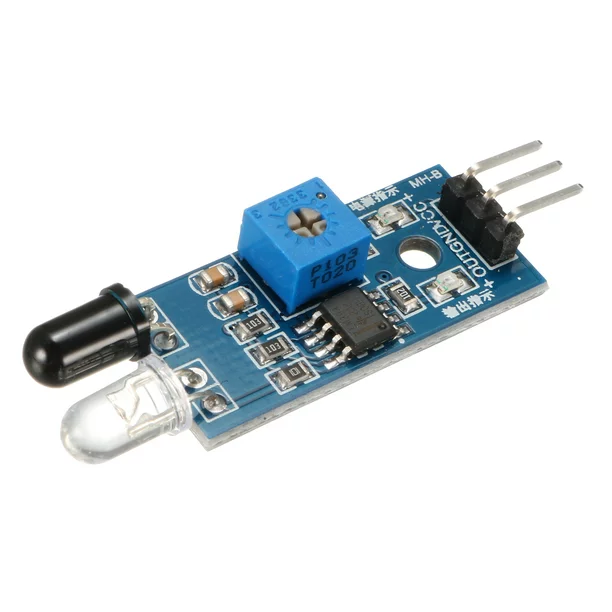
\includegraphics[width=0.5\linewidth]{IR.png}
    \caption{IR sensor}
    \label{fig:enter-label}
\end{figure}
An IR sensor or Infrared Sensor is an electronic device which transmit in order to sense some perspective of the surroundings. It can measure the heat of an object.This sensors only measure infrared radiation. These types of radiations are invisible to our eyes, which can be detected by an infrared sensor. When IR light falls on the photodiode, the resistances and the output voltages will change in proportion to the magnitude of the IR light received. Active infrared sensors work with radar technology and they both emit and receive infrared radiation. The sensor can not only detect movement in an environment but also how far the object is from the device.[6]

\subsection{Rain Sensor}
 A rain sensor is a switching device that is used to detect the rainfall. It works like a switch and the principle of working of this sensor is, whenever there is rain, the switch will be normally closed. This sensor detects the rain and gives an alert to concerned persons in different fields like irrigation, home automation, automobile communucation etc. It measures the moisture via analog output pins and it provides a digital output when a threshold of moisture exceeds.
 \begin{figure}
     \centering
     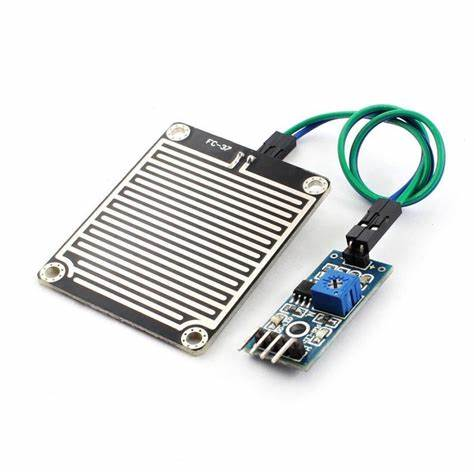
\includegraphics[width=0.5\linewidth]{rainsensor.png}
     \caption{ rainsensor}
     \label{fig:enter-label}
 \end{figure}

\section{Implementation}

Here we provide you the implementation of our project.

\begin{enumerate}
    \item Automate pitch covering: 
    
   When rain started Humidity Detection sensor detect rain it send reading to the Arduino and Arduino command the stepper motor to proceed. 
    
    
    Humidity Detection Sensor  -----Arduino Uno ------ Stepper Motor -----Cover Mechanism
    
    Humidity Detection Sensor: 
Detect when rain started.
    
    Aurduino Uno:
    
   Read analog signal from sensor and analize reading.
    
    Stepper Motor:
    
    After receiving signal from aurduino motor takes the commandig steps.
    
    
    \item Automated Boundary Line fixing: 
    
   Weight sensor ------- Auruino Uno ------ DC motor ------ Mechanism
    
    Weight Sensor: Sense the rope weight 
    
    Aurduino Uno:
    
    Receiving signal from weight sensor and give instruction to DC Motor.
    
    DC Motor:
    
    After receiving signal from  DC Motor follow command. 
    
    \item Power Play Player Count:
    
    IR Sensor----Arduino----Display
    
    IR Sensor:
 IR senor count from the start and sending signal to arduino.
    Arduino Uno:
    
    After getting signal, Arduino will show in LCD.
    
  .LCD Display: Receiving command from Arduino.
    
    \item Maximum Sunlight absolve system:

LDR Sensor ---- Arduino Uno----- Servo Motor

LDR Sensor : Light Detection Photosensitive send analog signal to Arduino.

Arduino Uno : Arduino Receive signal from LDR and send command to Servo Motor.

Servo Motor: Servo Motor receive signal from Arduino.

\item Automated Light Brightness Increase And Decrease:

LDR ---- Arduino Uno--- LED Light

LDR Sensor : Light Detection Photosensitive send analog signal to Arduino.

Arduino Uno : Arduino Receive signal from LDR and send command to LED Light.

LED Light: LED light Ingres or decrease brightness according Arduino Signal.
 
    
\end{enumerate}












\begin{thebibliography}{00}


\bibitem{b1} https://docs.arduino.cc/hacking/software/PortManipulation

\bibitem{b2} 
Servo Motor Basics, Working Principle & Theory (circuitdigest.com)

\bibitem{b3} https://www.sciencedirect.com/topics/materials-science/humidity-sensor


\bibitem{b4} 
https://en.wikipedia.org/wiki/DC_motor
  
     https://en.wikipedia.org/wiki/Lithium-ion_battery
 
     https://www.elprocus.com/infrared-ir-sensor-circuit-and-working/

\end{thebibliography}





\end{document}
